\documentclass[emulatestandardclasses]{scrartcl}
\usepackage{graphicx}
\usepackage{color}
\usepackage[ngerman]{babel}
\usepackage{hyperref}
\usepackage{fullpage}
\usepackage[utf8]{inputenc}
\usepackage{calc} 
\usepackage{enumitem}
\usepackage{titlesec}
\newcommand{\todo}[1]{\textcolor{red}{TODO: #1}\PackageWarning{TODO:}{#1!}}
\date{\vspace{-3ex}}
\begin{document}

\title{
	\includegraphics*[width=0.75\textwidth]{ErstesSem/images/hu_logo.png}\\
	\vspace{24pt}
	Plato's Phaedo}
\subtitle{\vspace{10pt}Proseminar WS 17/18\\
          David Ebrey\\
          Philosophisches Institut I \\ 
          Humboldt Universit"at zu Berlin}
\author{Lennard Wolf\\
        \small{\href{mailto:lennard.wolf@student.hu-berlin.de}{lennard.wolf@student.hu-berlin.de}}}
\maketitle
\begin{abstract}
In this seminar we will carefully work through Plato's Phaedo, which discusses ethical, epistemological, and metaphysical ideas that at the heart of Plato’s philosophy. Topics covered include: causation, the nature of the soul, the problems caused by the body, how inquiry is possible, the proper attitude and methodology for inquiry, why (and in what sense) the forms are distinct from sensible things, and why the best life is spent contemplating the forms. We will also discuss how the literary elements of the dialogue are related to its philosophical ideas.
The seminar will be in English and will assume basic familiarity with Plato's works. Knowledge of Greek is not required, but we will occasionally discuss the Greek, as needed.
\end{abstract}
\newpage

\tableofcontents
%\listoffigures
\newpage


\section{Introduction\\(19.10.17)}

\begin{itemize}
  \item Reading: Phaedo until next week
  \item Should read Laches before!
  \item Ecthyphro would be good 
  \item laches authyphro cooper
  \item Apology!!
  \item every week one page assignment to write what is confusing you?
  \item 15 to 20 pages! during the semester meeting! what is the central question to answer in the paper? how to go about it? hand in draft by March 15!
  \item apology, laches, phaedo 
  \item The early/Socratic dialogues: Laches, Euthyphro, Apology
  \item "`Unfolding Struucture"' of the dialogue: some claims are explained later in the text, but not explicitly!
  \item What is it? $\rightarrow$ "`Form"' 
\end{itemize}


\subsection{Apologie}

\begin{itemize}
  \item Werde anders sprechen als vllt erwartet
  \item Gegen zwei Klagen muss verteidigt werden: 1. alte Beschuldigungen, die schon lange herrschen: er treibe Naturphilosophie und darauf basierende Verleumdungen, er argumentiere ohne Rücksicht auf Wahrheit, 2. neue Klagen, eben erst vorgetragen, er lehre diese Dinge für Geld (Meletos)
  \item Klage: "`Sokrates tut Unrecht und treibt Unnützes, indem er erforscht, was unter der Erde und am Himmel ist, die schwächere Rede zur stärkeren macht, und dies auch unterrichtet."'
  \item Zur Verteidigung will er von altem Vorurteil befreien
  \item Verteidigung: Ich habe nichts dergleichen getan, fragt euch gegenseitig als Zeugen, niemand wird so etwas behaupten (?) $\rightarrow$ aber warum wird dann geklagt und warum spricht niemand dagegen?
  \item Orakel von Delphi: Sokrates ist intelligentester von allen $\rightarrow$ was heißt das?
  \item Geht zu scheinbar klugem Politiker um ihm zu zeigen, er sei nicht so klug wie er denkt, doch das hat ihn nur verhasst gemacht
  \item Beide wissen nichts, doch Unterschied: der andere glaubt etwas zu Wissen, Sokrates nicht
  \item Ich bin darum klüger "`dass ich, was immer ich nicht weiß, auch nicht zu wissen glaube."'
  \item Dieses Unwissen lehrt er, im Namen des Gottes
  \item Du jungen Leute folgen ihm und ahmen ihm nach, die anderen zu prüfen
  \item Die Leute werden zornig und meinen, Sokrates verzöge die Jugend
  \item Daher klagen sie ihn nun an (Ende Verteidigung 1)
  \item Meletos: interessiere sich gar nicht für die Jugend, da er sich nie gefragt hat, wer sie wie bessern könne
  \item Niemand will sich selbst schaden, also kann er die Jugend nicht absichtlich verderben, da ihm sonst Schaden zukommt, also muss er es, wenn er es tut, unabsichtlich tun
  \item Das Gesetz sagt, dass so einem Menschen nur im Privaten auf die Finger gehauen werden soll \emph{schlechtes Argument, damit wäre jeder Täter unschuldig}
  \item Frage: \emph{wie} wird die Jugend verdorben? Klage: Gottlosigkeit und Dämonenglaube
  \item Sokrates zeigt Widerspruch, denn um Dämonendinge zu lehren kann er nicht gottlos sein (Ende Verteidigung 2)
  \item Doch was ihn zu Fall bringen wird sind nicht die Klagen, sondern die Missgunst der Masse
  \item Schämst du dich nicht Dinge zu tun, die dich in Gefahr bringen? - Dann wären auch die Heroen von Troja unwürdig. Die Schande ist doch schlimmer als der Tod!
  \item Die Angst vor dem Tode setzt den Glauben voraus, der Tod sei das schlimmste!
  \item "`Mein Bester, du bist Athener, ein Bürger der größten und durch Bildung und Macht berühmtesten Stadt, und du schämst dich nicht, dich darum zu kümmern, wie du zu möglichst viel Geld und wie du [e] zu Ehre und Ansehen kommst, doch um die Vernunft und die Wahrheit und darum, dass du eine möglichst gute Seele hast, kümmerst und sorgst du dich nicht?"'
  \item Selbst wenn ihr mich freisprecht, ich werde immer dem Gott dienen und mich und die anderen zu Erkenntnis bewegen. Wenn ihr mich tötet schadet ihr euch mehr als mir.
  \item Die Kläger konnten keine Zeugen bringen, und dass Sokrates Geld nähme, dagegen ist seine Armut ein Zeuge
  \item War nie politisch aktiv, denn so ungerecht die Umstände auch sind, sie würden ihn nie dazu geleiten, Dinge gegen Gott zu tun (Scheiben einwerfen)
  \item Sokrates habe nie gelehrt, doch wenn einer zuhören will, so verwehrt er es ihm auch nicht
  \item Ende: Ich werde nicht flehen und bitten und Mitleid erzeugen, dies wäre nicht rechtens. Vielmehr wollte ich informieren und überzeugen.
  \item ---- Ende Erste Rede ----
  \item Stellt Antrag auf Speisung im Prytaneion (wurde für besondere Verdienste gewährt und entspricht nach heutigen Vorstellungen der Verleihung einer Ehrenbürgerwürde)
  \item Denn andere Anträge sind unsinnig. Verbannung würde ihn nur in andere Städte schicken und sich alles im Kreis drehen. 
  \item "`Warum nicht mit dem Fragen aufhören?"' - "`Ich muss Gott folgen. ein Leben ohne Prüfung ist für den Menschen nicht lebenswert."'
  \item Antrag auf Geld: Platon et al als Bürgen
  \item ---- Ende Zweite Rede ----
  \item Lieber mit ehrenvoller Verteidigung zugrundegehen, als mit jammernder am Leben bleiben.
  \item Die Richter meinen ihm zu schaden mit der Strafe, doch ist doch vollkommen unklar, was im Tod wirklich passiert. 
  \item Vielleicht ist der Tod ein ruhiger Schlaf - vielleicht trifft er auf die Heroen im Hades.
  \item Ob der Tod oder das Leben das bessere Los ist, das weiß nur der Gott.
  \item ---- Ende Dritte Rede ----
\end{itemize}

\subsection{Laches}

\begin{itemize}
  \item Melesias und Lysimachos fragen Nikias und Laches um Rat bei der Erziehung der Söhne
  \item Diese schlagen SOkrates noch vor, dieser wird nach ihnen reden und ergänzen
  \item Nikias: Muße ist so wichtig wie körperliche Tüchtigkeit; Fechten ist gut zu lernen, denn es macht nicht nur tüchtig und mutig für den Kampf, sondern verleiht auch beeindruckendes Aussehen
  \item Laches: Aber alles zu lernen ist doch gut. Zudem: persönlliche Erfahrung mit Fechtern eher negativ. Stellen mehr ihre Fähigkeiten zur Schau, doch wenig praktischen Wert (umgehen echte Kämpfe). Daher nicht zu empfehlen.
  \item Sokrates: Ich hatte keiner Lehrer darin und habe auch keine Kenntnisse, doch die beiden schon. Daher bin ich verwirrt ob ihres Widerspruchs. Wen kennt ihr der gelehrt hat und wen habt ihr gelehrt, sodass ihr denn befugt seit, die ursprüngliche Frage zu beantworten? 
  \item Nikias sagt er lässt sich gern von Sokrates ausfragen, Laches meint er vertraut ihm da er sich im Krieg verdient gemacht hat. (Realisation: es wird wohl um die Väter gehen, nicht um die Bildung der Söhne)
  \item Sokrates: Um zu sagen, ob etwas gut gelehrt wird, müssen wir es selber können. Um also über die Lehre der Tugend zu beraten, müssen wir selbst in der Tugend gelehrt sein. Wir müssen also wohl Tugend kennen. Beginnen wir also mit Tapferkeit. Was ist das?  
  \item Erste Antwort zu speziell, Sokrates will allgemeine: Beharrlichkeit der Seele? Nein! Beharren auf Unwissen ist nicht rechtens. $\rightarrow$ es zeigt sich dass sie gar nicht wissen was das eigentlich ist
  \item Befragen Nikias: Tapferkeit ist eine Art Wissen: Wissen darum, was Furcht und Zuversicht bewirken (...Gelaber...)
  \item Sokrates: dieses Wissen wäre eher die Tugend selber, und so ist Nikias übers Ziel hinaus geschossen (nicht ganz verstanden)
  \item Ende: Wird Sokrates sich um die Tüchtigkeit der Söhne kümmern: Nein, denn ich bin ja so ratlos wie ihr auch. Wir sollten selber alle nochmal zur Schule gehen.
\end{itemize}


\subsection{Phaidon}

\begin{itemize}
  \item Sokrates konnte noch länger leben, weil eine Zeremonie noch abgeschlossen werden musste
  \item Sokrates: das Angenehme und Schmerzliche sind so verheiratet, dass es das eine ohne das andere gar nicht gibt
  \item Sokrates hat gedichtet. Warum: Weil die Götter es ihm im Traum schon immer sagten. Er tat es bisher nicht, da er meinte die Philosophie sei die höchste Form der Muße. Doch er schien sich zu irren (?) und so muss er seiner Pflicht nachgehen
  \item Warum sollten Philosophen ihm nicht folgen und sich Gewalt antun? Denn für einige wäre der Tod sicher besser als das Leben. - Weil die Menschen nicht sich selbst gehören, sondern den Göttern!
  \item \textbf{Erster Einwand: Wieso hängen die Vernünftigsten dann am wenigsten von allen am Leben?}
  \item Einwand von Kebes: Wenn das so wäre, dann müssten doch die Vernünftigsten am meisten am Leben hängen. Doch es ist genau umgekehrt, und die Vernünftigsten sehnen sich glatt zum Suizid, die Masse aber will leben.
  \item Daher muss Sokrates sich noch einmal besser verteidigen als vor Gericht!
  \item Sokrates: Glaubt zu besseren Göttern (und Menschen) zu kommen, da er Leben mit Philosophie verbracht hat.
  \item Die die sich mit Philosophie befassen, tun nichts anderes als zu sterben und tot zu sein.
  \item Packmeinung: Philosophen wünschen zu sterben, verdienen den Tod. Doch inwiefern und welchen Tod? 
  \item Simmias: Tod: Trennung der Seele vom Körper; Tot-Sein: Körper abgesondert ganz für sich
  \item Philosophen wollen so weit wie möglich weg von den fleischlichen, körperlichen Bedürfnissen und sich der Seele zuwenden $\rightarrow$ Mögliche Folge: Solch einer wäre doch froh tot zu sein
  \item Der Körper wird aber als Werkzeug herangezogen, dieser ist aber ein nicht sonderlich gut im Wahrnehmen. Wann erfaßt Seele Wahrheit? Wenn sie vom Körper in Ruhe gelassen wird und denken kann.
  \item Das Gerechte, das Gute und das Schöne existieren, aber sind nicht Seiendes, und werden von der Seele nur wahrgenommen; Das Seiende wird vom Körper wahrgenommen
  \item Solang wir den Körper haben, können wir das Wahre nicht erreichen. So gibt es zwei Möglichkeiten: Entweder wir werden das Wahre \emph{nie} erreichen, oder erst nach dem Tode.
  \item Ein zum Tode verurteilter, der dazu unwillig ist, ist kein Liebhaber der Wahrheit, sondern des Körpers
  \item Tod is größtes Übel. Tapfere Erdulden Tod vor Angst vor etwas schlimmeren (?). Daher: Tapfer wegen Angst?  
  \item Man kann aus Zügellosigkeit dem einen gegenüber besonnen einem anderen gegenüber sein
  \item Diese Beispiele können doch nicht wahre Tugend sein!
  \item Das Wahre ist eine Reinigung von alledem; und das tugendhafte also ist auch immer reinigend
  \item Wegen alledem sorgt sich Sokrates nicht vor dem Tod, denn es wird sich zeigen, ob er nicht sogar das Wahre treffen wird 
  \item \textbf{Zweiter Einwand: Woher wissen wir, dass die Seele nach dem Tode weiter existiert?}
  \item Einwand von Kebes: Was, wenn die Seele nach dem Tod zugrundegeht und nichts und nirgendwo mehr ist? Was ist deine Meinung dazu?
  \item Eine Möglichkeit: Die Lebenden kommen eh von den Toten.
  \item Entsteht alles, das ein Gegenteil hat, aus diesem Gegenteil? Aber dieser Werdegang ist in sich ein einzelnes (Wachsen, Schrumpfen etc) $\rightarrow$ Daher: ebenso bei Leben und Tot-Sein
  \item Damit aus den Toten die Lebenden kommen können, müssen die Seelen irgendwo sein!
  \item Andere Möglichkeit:
  \item Wenn es Dinge gäbe, die nicht gegenteilig sind, so müssten diese auf Dauer an der einen Stelle zusammenlaufen. Dann könnte es doch zum Beispiel kein Lebendiges mehr geben irgendwann!
  \item Kebes: So ließe sich auch erklären, dass wir in der Erkenntnis uns nur erinnern
  \item Wenn man sich erinnert, muss man es vorher schon gekannt haben. Erinnerung entsteht durch ähnliche wie auch unähnliche (bloß assoziierte Dinge) Das Gleiche als solches gibt es, doch es ist nicht dasselbe wie die gleichen Dinge
  \item Und als wir das erste Mal gleiche Dinge sahen, so waren wir an Das Gleiche erinnert (?)
  \item Und die Erkenntnis der Gleichheit müssen wir also schon vor der Wahrnehmung gehabt haben, also vor der Geburt! 
  \item Die Seele existiert also schon vor der Geburt - (Dieser Schritt war wohl nötig um den Einwand tatsächlich zu beantworten)
  \item \textbf{"`Dritter"' Einwand: Woher wissen wir, dass die Seele nach dem Tode weiter existiert?}
  \item  
\end{itemize}

\textbf{Notizen}

\begin{itemize}
  \item Er will zum einen sagen dass man sich nicht umbringen solle, und zum anderen, dass es besser für ihn sein wird nach dem Tode (??)
  \item Das \emph{Schöne} nimmt mein Körper doch wahr..?
  \item 69b: was rein gemacht wird wird auch wieder unrein, so kann sich die tugend gegen sich selbst tauschen..?
  \item 
\end{itemize}

\textbf{Questions to the text}

\begin{itemize}
  \item 68d: not brave because of fear! weird argument?
  \item Why is the true philosopher in Death in a better position that the layman?
  \item Why is it so easily dismissed, that at some point there might be no living being anymore?
  \item Socrates says he knows nothing, but in Phaedo he shows routes of thinking which are clearly not necessarily true. He seems to uphold certain information, to show why he knows things.. or not?
\end{itemize}

\section{Second Week \\(26.10.17)}

\subsection{Initiation passage}

\begin{itemize}
  \item Hades is the unseen
  \item Peoples claims about afterlife are correct, but, in which way?
  \item Purification is leaving behind bodily pleasures
  \item True initiates are those, that pursue philosophy in the right way
  \item philosophy as a process of initiation, in which certain deeper and deeper truths are revealed
  \item Structure of the dialogue: Starting out with the common view of the world, from which we are freed, and thus initiated
  \item Socrates compared to heroes
  \item Ordinary and Extraordinary are often contrasted, e.g.: beginning: geographic locations of people, later: how clear the souls are 
  \item 
\end{itemize}


\newpage
%\section{"Uber den Professor}
%Matthias Schlo"sberger ist Heisenbergstipendiat der Deutschen Forschungsgemeinschaft
%an der Humboldt Universit"at zu Berlin mit dem Forschungsprojekt "`Die Erfahrung der Realit"at durch Widerstand"'.
%
%\begin{figure}[h]
%	\centering
%	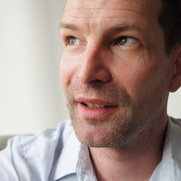
\includegraphics[width=0.3\textwidth]{images/Matthias_Schlossberger.png}
%	\caption{Matthias Schlo"sberger}
%	\label{fig:MS}
%\end{figure}


%\begin{figure}[h]
%	\centering
%	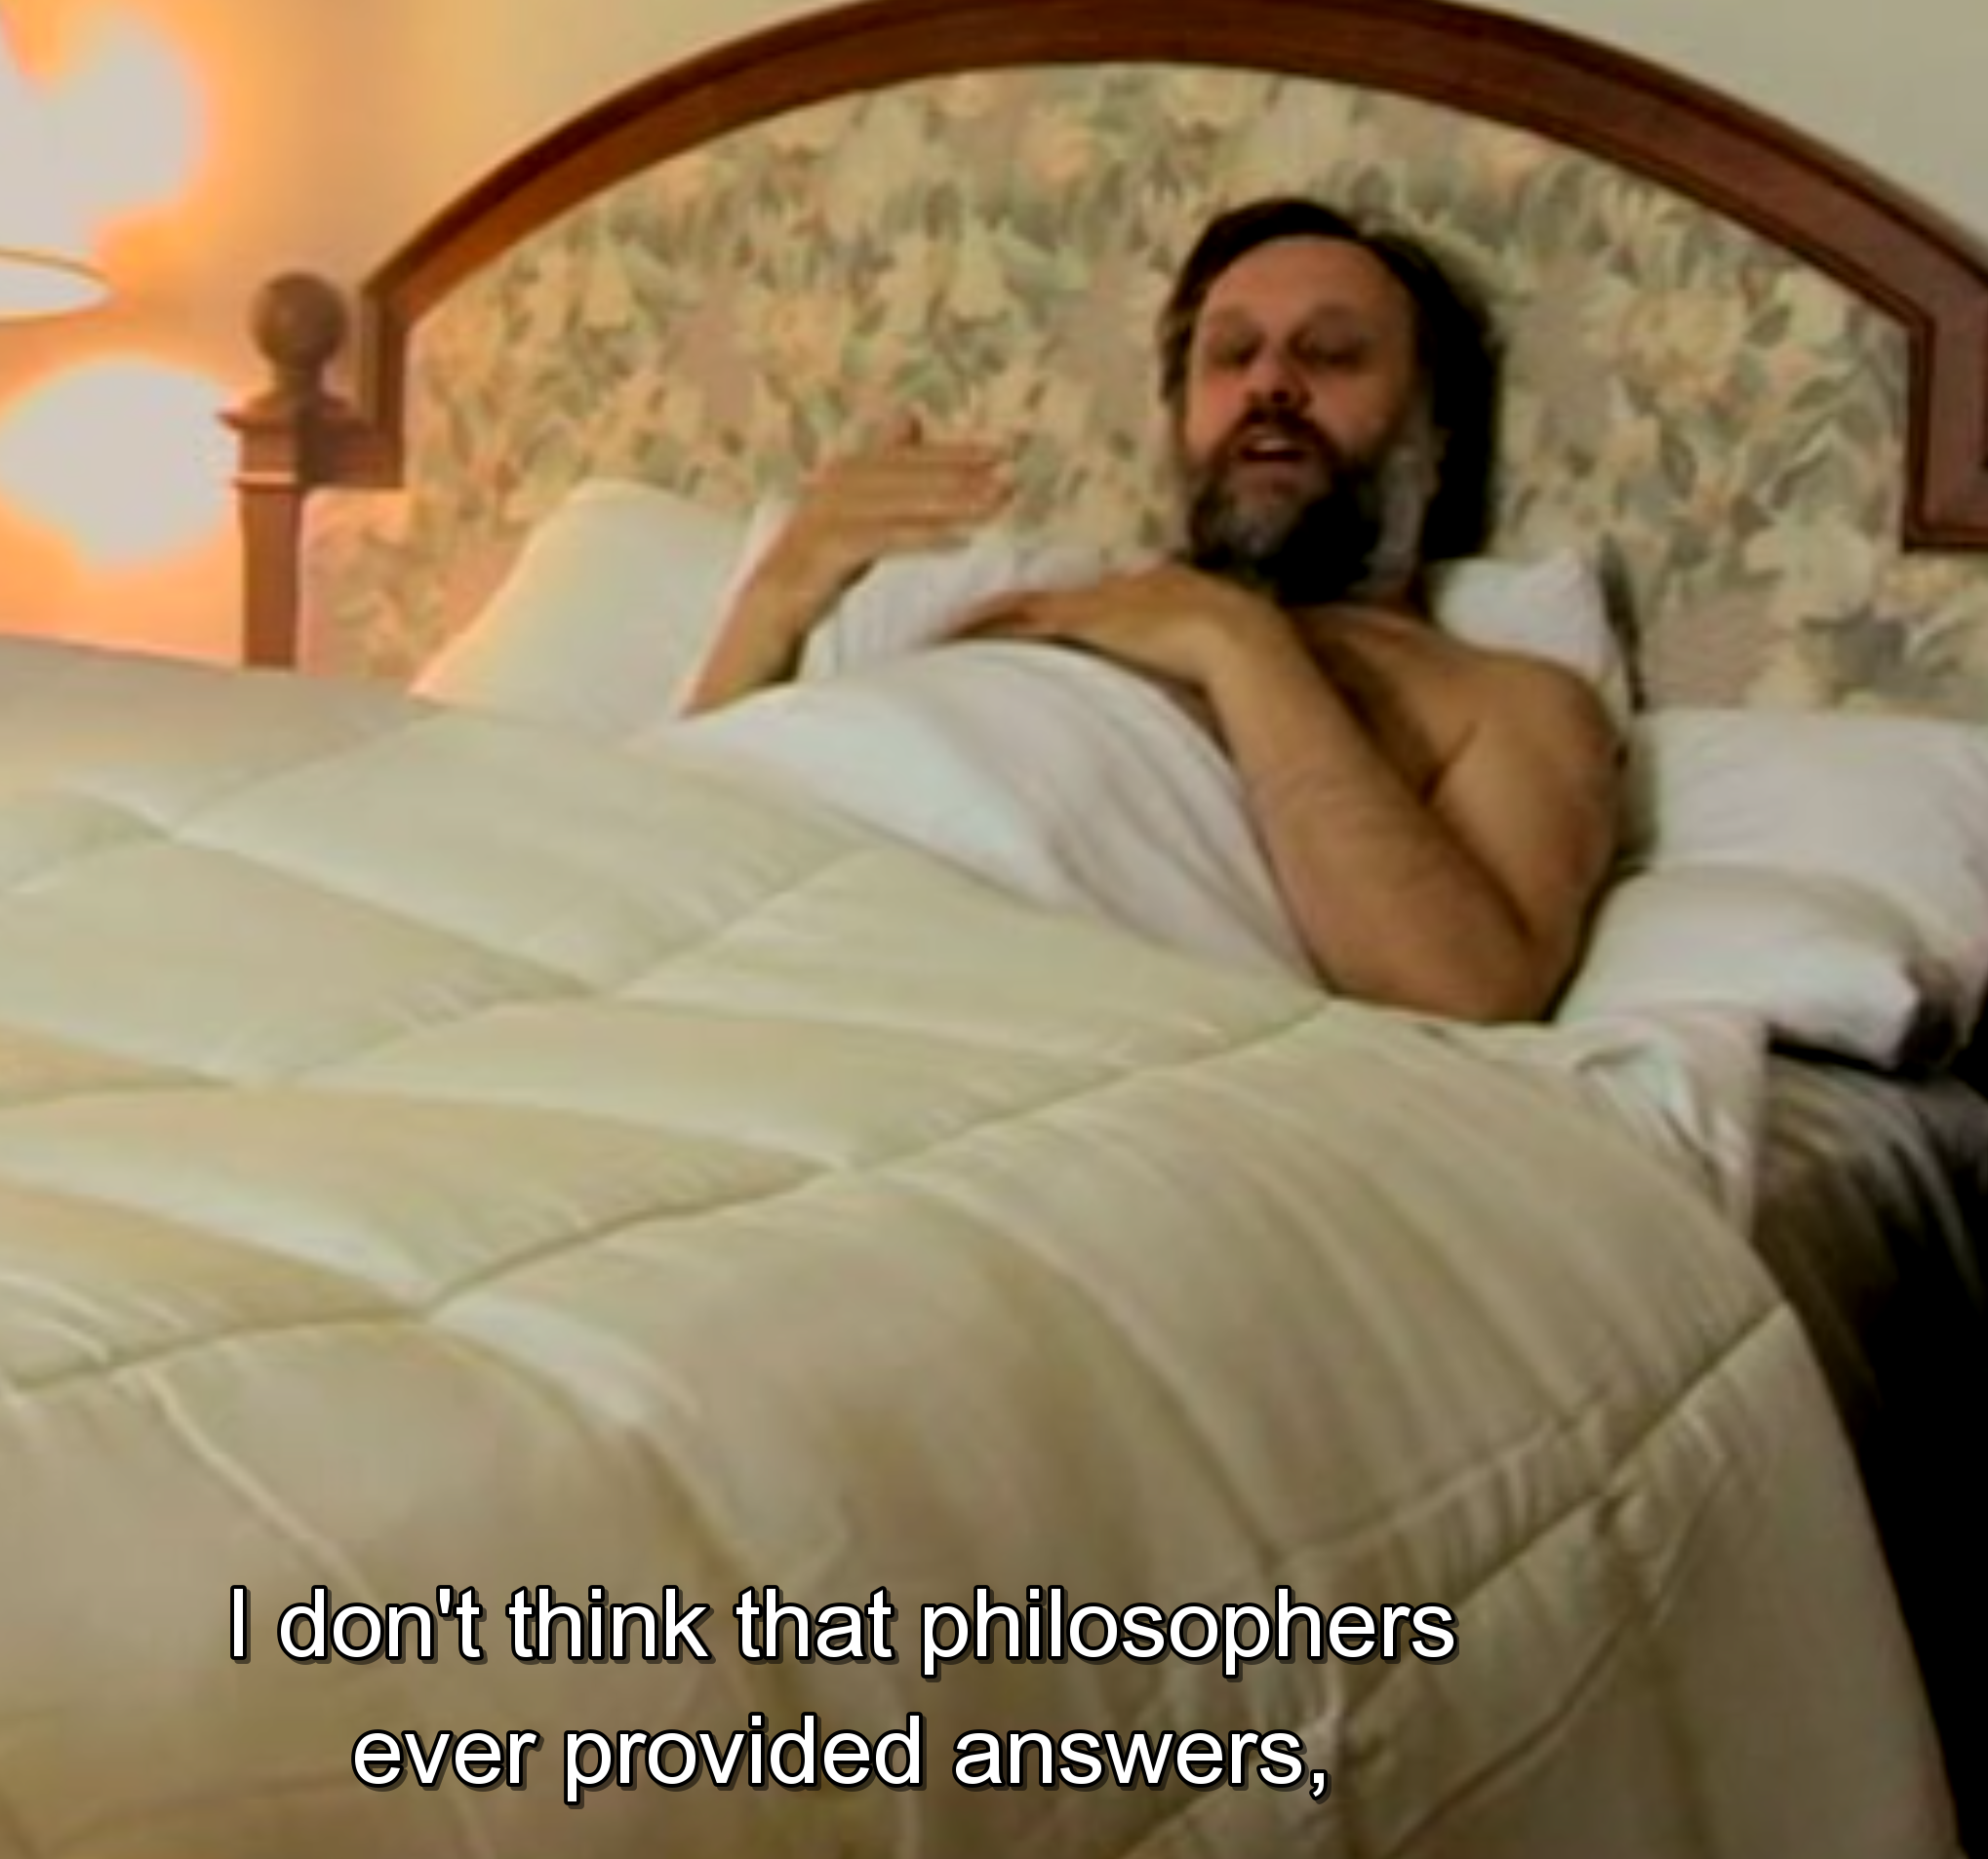
\includegraphics[width=0.5\textwidth]{images/template.png}
%	\caption{Template Bild}
%	\label{fig:template}
%\end{figure}

\end{document}
